\documentclass[twoside]{book}

% Packages required by doxygen
\usepackage{fixltx2e}
\usepackage{calc}
\usepackage{doxygen}
\usepackage[export]{adjustbox} % also loads graphicx
\usepackage{graphicx}
\usepackage[utf8]{inputenc}
\usepackage{makeidx}
\usepackage{multicol}
\usepackage{multirow}
\PassOptionsToPackage{warn}{textcomp}
\usepackage{textcomp}
\usepackage[nointegrals]{wasysym}
\usepackage[table]{xcolor}

% Font selection
\usepackage[T1]{fontenc}
\usepackage[scaled=.90]{helvet}
\usepackage{courier}
\usepackage{amssymb}
\usepackage{sectsty}
\renewcommand{\familydefault}{\sfdefault}
\allsectionsfont{%
  \fontseries{bc}\selectfont%
  \color{darkgray}%
}
\renewcommand{\DoxyLabelFont}{%
  \fontseries{bc}\selectfont%
  \color{darkgray}%
}
\newcommand{\+}{\discretionary{\mbox{\scriptsize$\hookleftarrow$}}{}{}}

% Page & text layout
\usepackage{geometry}
\geometry{%
  a4paper,%
  top=2.5cm,%
  bottom=2.5cm,%
  left=2.5cm,%
  right=2.5cm%
}
\tolerance=750
\hfuzz=15pt
\hbadness=750
\setlength{\emergencystretch}{15pt}
\setlength{\parindent}{0cm}
\setlength{\parskip}{3ex plus 2ex minus 2ex}
\makeatletter
\renewcommand{\paragraph}{%
  \@startsection{paragraph}{4}{0ex}{-1.0ex}{1.0ex}{%
    \normalfont\normalsize\bfseries\SS@parafont%
  }%
}
\renewcommand{\subparagraph}{%
  \@startsection{subparagraph}{5}{0ex}{-1.0ex}{1.0ex}{%
    \normalfont\normalsize\bfseries\SS@subparafont%
  }%
}
\makeatother

% Headers & footers
\usepackage{fancyhdr}
\pagestyle{fancyplain}
\fancyhead[LE]{\fancyplain{}{\bfseries\thepage}}
\fancyhead[CE]{\fancyplain{}{}}
\fancyhead[RE]{\fancyplain{}{\bfseries\leftmark}}
\fancyhead[LO]{\fancyplain{}{\bfseries\rightmark}}
\fancyhead[CO]{\fancyplain{}{}}
\fancyhead[RO]{\fancyplain{}{\bfseries\thepage}}
\fancyfoot[LE]{\fancyplain{}{}}
\fancyfoot[CE]{\fancyplain{}{}}
\fancyfoot[RE]{\fancyplain{}{\bfseries\scriptsize Generated by Doxygen }}
\fancyfoot[LO]{\fancyplain{}{\bfseries\scriptsize Generated by Doxygen }}
\fancyfoot[CO]{\fancyplain{}{}}
\fancyfoot[RO]{\fancyplain{}{}}
\renewcommand{\footrulewidth}{0.4pt}
\renewcommand{\chaptermark}[1]{%
  \markboth{#1}{}%
}
\renewcommand{\sectionmark}[1]{%
  \markright{\thesection\ #1}%
}

% Indices & bibliography
\usepackage{natbib}
\usepackage[titles]{tocloft}
\setcounter{tocdepth}{3}
\setcounter{secnumdepth}{5}
\makeindex

% Hyperlinks (required, but should be loaded last)
\usepackage{ifpdf}
\ifpdf
  \usepackage[pdftex,pagebackref=true]{hyperref}
\else
  \usepackage[ps2pdf,pagebackref=true]{hyperref}
\fi
\hypersetup{%
  colorlinks=true,%
  linkcolor=blue,%
  citecolor=blue,%
  unicode%
}

% Custom commands
\newcommand{\clearemptydoublepage}{%
  \newpage{\pagestyle{empty}\cleardoublepage}%
}

\usepackage{caption}
\captionsetup{labelsep=space,justification=centering,font={bf},singlelinecheck=off,skip=4pt,position=top}

%===== C O N T E N T S =====

\begin{document}

% Titlepage & ToC
\hypersetup{pageanchor=false,
             bookmarksnumbered=true,
             pdfencoding=unicode
            }
\pagenumbering{alph}
\begin{titlepage}
\vspace*{7cm}
\begin{center}%
{\Large My Project }\\
\vspace*{1cm}
{\large Generated by Doxygen 1.8.14}\\
\end{center}
\end{titlepage}
\clearemptydoublepage
\pagenumbering{roman}
\tableofcontents
\clearemptydoublepage
\pagenumbering{arabic}
\hypersetup{pageanchor=true}

%--- Begin generated contents ---
\chapter{Hierarchical Index}
\section{Class Hierarchy}
This inheritance list is sorted roughly, but not completely, alphabetically\+:\begin{DoxyCompactList}
\item Q\+Object\begin{DoxyCompactList}
\item \contentsline{section}{Client}{\pageref{class_client}}{}
\end{DoxyCompactList}
\end{DoxyCompactList}

\chapter{Class Index}
\section{Class List}
Here are the classes, structs, unions and interfaces with brief descriptions\+:\begin{DoxyCompactList}
\item\contentsline{section}{\mbox{\hyperlink{class_client}{Client}} \\*Classe décrivant un client. Le client a pour rôle d\textquotesingle{}envoyer un message au serveur }{\pageref{class_client}}{}
\end{DoxyCompactList}

\chapter{File Index}
\section{File List}
Here is a list of all documented files with brief descriptions\+:\begin{DoxyCompactList}
\item\contentsline{section}{E\+:/\+B\+T\+S/\+S\+N2/\+Angibaud/\+T\+P\+\_\+\+S\+O\+C\+K\+E\+T\+\_\+\+C\+L\+I\+E\+N\+T/\mbox{\hyperlink{client_8h}{client.\+h}} \\*Fichier de déclaration de la classe client }{\pageref{client_8h}}{}
\end{DoxyCompactList}

\chapter{Class Documentation}
\hypertarget{class_client}{}\section{Client Class Reference}
\label{class_client}\index{Client@{Client}}


Classe décrivant un client. Le client a pour rôle d\textquotesingle{}envoyer un message au serveur.  




{\ttfamily \#include $<$client.\+h$>$}

Inheritance diagram for Client\+:\begin{figure}[H]
\begin{center}
\leavevmode
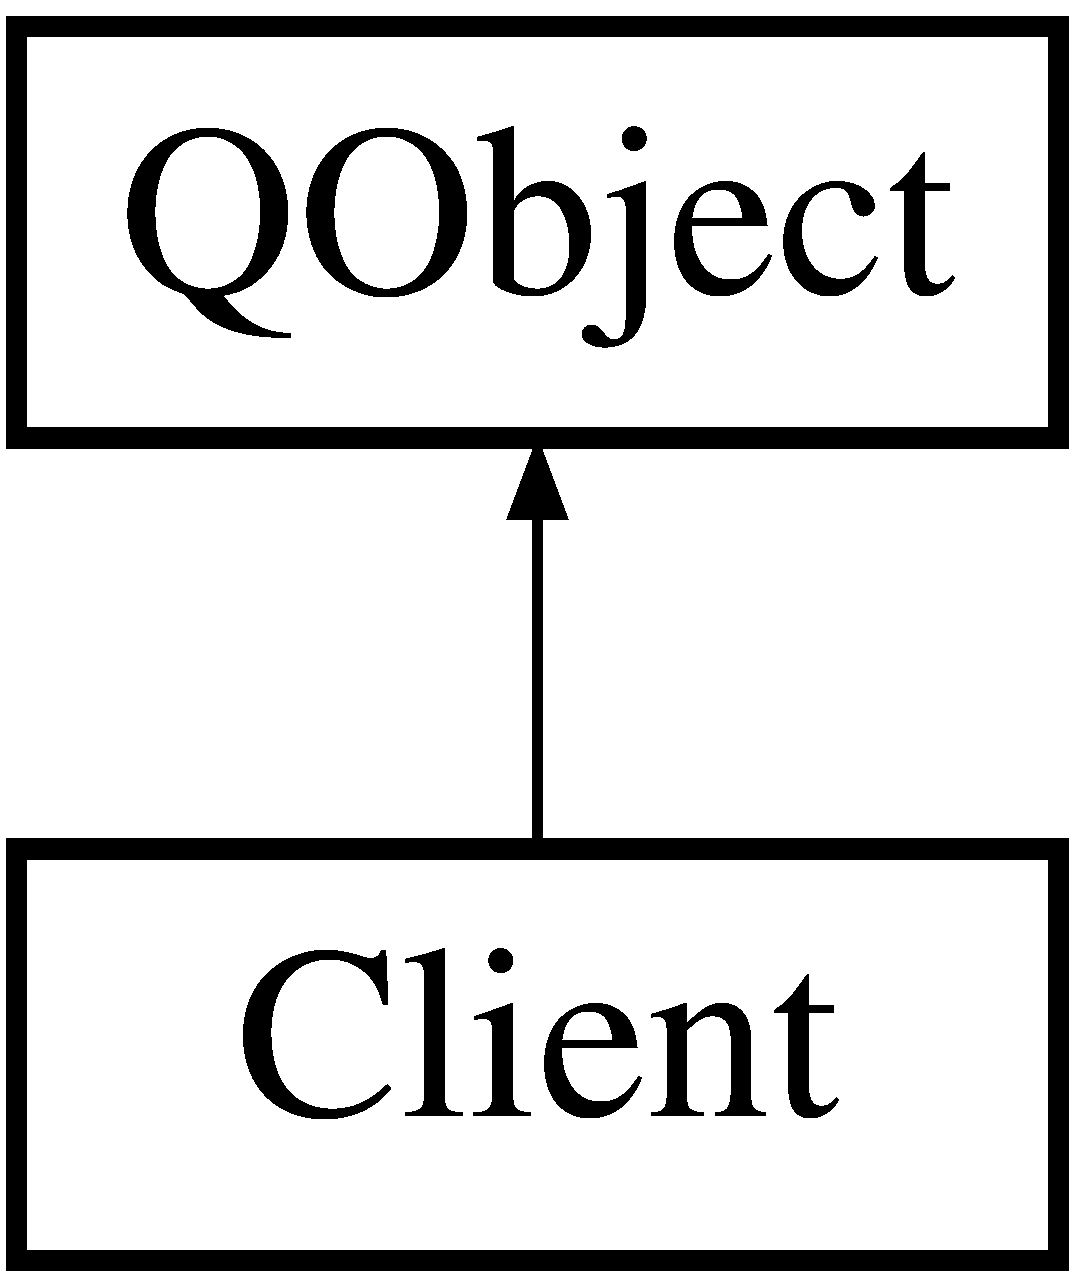
\includegraphics[height=2.000000cm]{class_client}
\end{center}
\end{figure}
\subsection*{Private Slots}
\begin{DoxyCompactItemize}
\item 
\mbox{\Hypertarget{class_client_ae5983d9d73779ff3a90acb1b73cf69cf}\label{class_client_ae5983d9d73779ff3a90acb1b73cf69cf}} 
void {\bfseries afficher\+Erreur} (Q\+Abstract\+Socket\+::\+Socket\+Error socket\+Error)
\end{DoxyCompactItemize}
\subsection*{Private Member Functions}
\begin{DoxyCompactItemize}
\item 
\mbox{\Hypertarget{class_client_ac55d565ea5da905ca3e3dea4da471a03}\label{class_client_ac55d565ea5da905ca3e3dea4da471a03}} 
void \mbox{\hyperlink{class_client_ac55d565ea5da905ca3e3dea4da471a03}{envoi\+Texte}} (const std\+::string \&s)
\begin{DoxyCompactList}\small\item\em Fonction permettant d\textquotesingle{}envoyer un message au serveur une fois la connexion établie. \end{DoxyCompactList}\end{DoxyCompactItemize}
\subsection*{Private Attributes}
\begin{DoxyCompactItemize}
\item 
\mbox{\Hypertarget{class_client_a7a4be02c7064314761fb11c2cf43c483}\label{class_client_a7a4be02c7064314761fb11c2cf43c483}} 
Q\+Tcp\+Socket $\ast$ \mbox{\hyperlink{class_client_a7a4be02c7064314761fb11c2cf43c483}{m\+\_\+tcp\+Socket}}
\begin{DoxyCompactList}\small\item\em Q\+Tcp\+Socket fournissant les paramètres nécessaires à l\textquotesingle{}établiseement d\textquotesingle{}une connexion avec le serveur sous forme d\textquotesingle{}objet. \end{DoxyCompactList}\item 
\mbox{\Hypertarget{class_client_af41d2cbd7c1a4c83c09599682ed358df}\label{class_client_af41d2cbd7c1a4c83c09599682ed358df}} 
Q\+Network\+Session $\ast$ \mbox{\hyperlink{class_client_af41d2cbd7c1a4c83c09599682ed358df}{m\+\_\+network\+Session}}
\begin{DoxyCompactList}\small\item\em Q\+Network\+Session permet de créer une session de communication avec le serveur sous forme d\textquotesingle{}objet. \end{DoxyCompactList}\end{DoxyCompactItemize}


\subsection{Detailed Description}
Classe décrivant un client. Le client a pour rôle d\textquotesingle{}envoyer un message au serveur. 

\begin{DoxyAuthor}{Author}
Alexandre Stanisiere 
\end{DoxyAuthor}


The documentation for this class was generated from the following files\+:\begin{DoxyCompactItemize}
\item 
E\+:/\+B\+T\+S/\+S\+N2/\+Angibaud/\+T\+P\+\_\+\+S\+O\+C\+K\+E\+T\+\_\+\+C\+L\+I\+E\+N\+T/\mbox{\hyperlink{client_8h}{client.\+h}}\item 
E\+:/\+B\+T\+S/\+S\+N2/\+Angibaud/\+T\+P\+\_\+\+S\+O\+C\+K\+E\+T\+\_\+\+C\+L\+I\+E\+N\+T/client.\+cpp\end{DoxyCompactItemize}

\chapter{File Documentation}
\hypertarget{client_8h}{}\section{E\+:/\+B\+T\+S/\+S\+N2/\+Angibaud/\+T\+P\+\_\+\+S\+O\+C\+K\+E\+T\+\_\+\+C\+L\+I\+E\+N\+T/client.h File Reference}
\label{client_8h}\index{E\+:/\+B\+T\+S/\+S\+N2/\+Angibaud/\+T\+P\+\_\+\+S\+O\+C\+K\+E\+T\+\_\+\+C\+L\+I\+E\+N\+T/client.\+h@{E\+:/\+B\+T\+S/\+S\+N2/\+Angibaud/\+T\+P\+\_\+\+S\+O\+C\+K\+E\+T\+\_\+\+C\+L\+I\+E\+N\+T/client.\+h}}


Fichier de déclaration de la classe client.  


{\ttfamily \#include $<$Q\+Tcp\+Socket$>$}\newline
{\ttfamily \#include $<$Q\+Object$>$}\newline
\subsection*{Classes}
\begin{DoxyCompactItemize}
\item 
class \mbox{\hyperlink{class_client}{Client}}
\begin{DoxyCompactList}\small\item\em Classe décrivant un client. Le client a pour rôle d\textquotesingle{}envoyer un message au serveur. \end{DoxyCompactList}\end{DoxyCompactItemize}


\subsection{Detailed Description}
Fichier de déclaration de la classe client. 

\begin{DoxyAuthor}{Author}
Alexandre Stanisiere 
\end{DoxyAuthor}

%--- End generated contents ---

% Index
\backmatter
\newpage
\phantomsection
\clearemptydoublepage
\addcontentsline{toc}{chapter}{Index}
\printindex

\end{document}
